\documentclass[aspectratio=43]{beamer}

\usepackage[T1]{fontenc}
\usepackage[utf8]{inputenc}
\usepackage[croatian]{babel}
\usepackage{tikz}


\usetikzlibrary{arrows.meta,trees}

\usetheme{Madrid}
\setbeamertemplate{navigation symbols}{}

\title{Kako računala igraju šah?}
\author{Matija Njegač}
\institute{PMF — MO}
\date{\today}

\begin{document}
	
	\begin{frame}
		\titlepage
	\end{frame}
	
	\begin{frame}{Antagonističke igre}
		\begin{itemize}
		\item Antagonističke igre su one koje se sastoje od dva ili više igrača imaju suprotne ciljeve. Pobjeda jednog igrača znači identičan i absolutni gubitak za ostale igrače.
		\item Primjeri: šah, križić kružić, go, shogi
		\end{itemize}
	\end{frame}
	
	\begin{frame}{Što je šahovska pozicija?}
		
		Koje uvjete trebamo zadovoljiti da jednoznačno definiramo
		šahovsku poziciju?
		\pause
		\vspace{0.5cm}
		
		\begin{columns}[T,onlytextwidth]
			
			\column{0.45\textwidth}
			\centering
			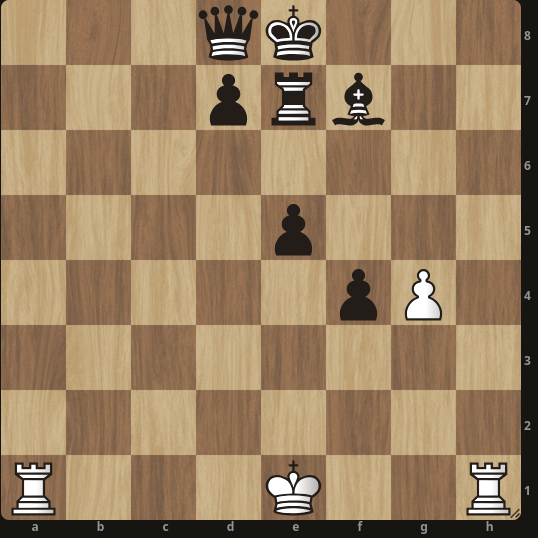
\includegraphics[width=\linewidth]{Pozicija1.png}
			
			\pause
			
			\column{0.52\textwidth}
			\begin{itemize}
				\item Položaj figura
				\pause
				\item Tko je na potezu
				\pause
				\item Jesu li se micali kralj ili topovi
				\pause
				\item Je li moguć en passant
				\pause
				\item Koliko poteza je prošlo od zadnjeg uzimanja figure
				ili pomicanja pješaka
			\end{itemize}
			
		\end{columns}
		Najčešći prikaz za zapis pozicije koji se koristi je FEN zapis
		
	\end{frame}
	
	\begin{frame}{Primjer šahovske pozicije}
		Primjer FEN zapisa:
		\texttt{\small 2r1k2r/1pQ1nppp/p1b1p1q1/8/4P3/2N1B1P1/PPPR1P1P/2KR4 b k - 0 15}
		
		\vspace{0.3cm}
		\centering
		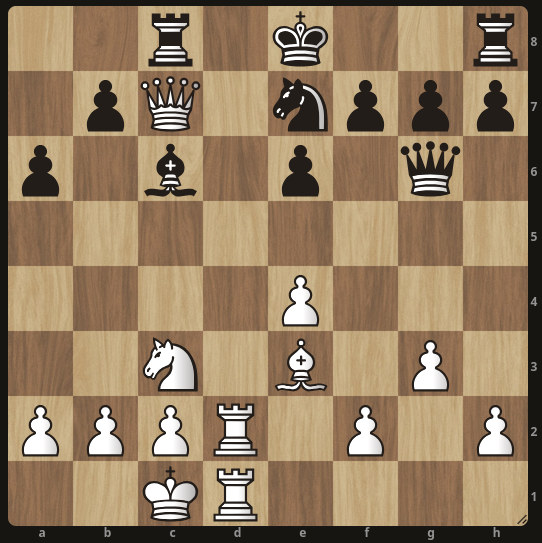
\includegraphics[height=0.55\textheight, keepaspectratio]{NjegTuksi.png}
		\pause
		\vspace{0.3cm}
		\\
		Njegač - Tuković Split 2021
	\end{frame}
	\begin{frame}{Pojednostavljeno stablo igre}
		\centering
		
		\begin{tikzpicture}[
			grow=down,
			level distance=17mm,
			level 1/.style={sibling distance=4cm},
			level 2/.style={sibling distance=2cm},
			position/.style={
				draw,
				rounded corners,
				align=center,
				font=\scriptsize,
				text width=2.7cm,
				inner sep=4pt
			},
			edge from parent/.style={draw, -{Stealth}}
			]
			\node[position] {Početna pozicija $P_0$\\
				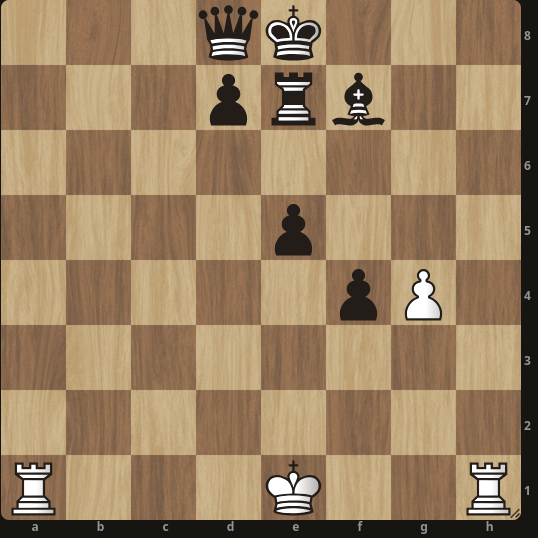
\includegraphics[width=1.1cm]{Pozicija1.png}\\
				Bijeli na potezu}
			child {
				node[position] {$P_1$\\nakon $1.\ g5$}
				child {
					node[position] {$P_2$\\nakon $1\ldots e4$}
				}
			}
			child {
				node[position] {$P_1$\\nakon $1.\ Rh8+$}
				child {
					node[position] {$P_2$\\nakon $1\ldots Bg8$}
				}
			}
			child {
				node[position] {$P_1$\\nakon $1.\ Ra8?$}
				child {
					node[position] {$P_2$\\nakon $1\ldots Qxa8$}
				}
			};
		\end{tikzpicture}
		
		\vspace{0.2cm}
		{\scriptsize Prikazani su samo odabrani potezi, ne sve legalne grane.}
	\end{frame}
	
	
	
	\begin{frame}{Minimax}
		Procjena pozicije kada je na potezu MAX:
		\[
		V(s) = \max_{s' \in \mathrm{Djeca}(s)} V(s')
		\]
	\end{frame}
	
\end{document}